\documentclass[../../thesis.tex]{subfiles}

\graphicspath{{./img/}}

\begin{document}


\section{Temporal Networks}
\label{sec: temporal_network}


Continuing our investigation, we modeled the Bitcoin transactions inputs and outputs addresses into a list of edges with timestamps. Then, this edge list can be seen as a graph that changes its edges over time. Hence, we shaped the Bitcoin transactions data into an instance of a Temporal Network \cite{temporalNetworks}.



Temporal Network is a type of network where edges are not continuously active. The edges have an extra attribute which tells \textit{when} this edge happened in time. On the contrary of traditional network theory, temporal network approaches target the analysis of information, about \textit{when} things happen. The motivation behind is the edge activations affect the dynamics of the network. Therefore, the central interest is the flow of information.


\begin{figure}
    \centering
    
    \begin{subfigure}{0.45\textwidth}
        \centering
        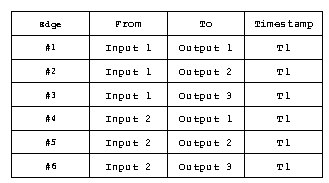
\includegraphics[width=0.9\textwidth]{content/unveiling/img/imput_solution_as_graph_edgelist}         
        \caption{The result of Figure~\ref{fig:inputSolution} as an edge list containing six edges with timestamps.}
        \label{fig:inputSolutionTableGraphA}
    \end{subfigure}\hfill
    \begin{subfigure}{0.45\textwidth}
        \centering
        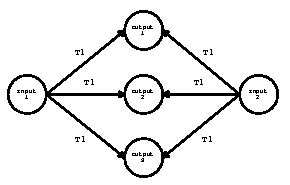
\includegraphics[width=0.9\textwidth]{content/unveiling/img/imput_solution_as_graph}         
        \caption{The result edge list (A) as a timestamped subgraph.}
        \label{fig:inputSolutionTableGraphB}
    \end{subfigure}

\caption{The example of converting the same transaction with two inputs and three outputs from Figure~\ref{fig:inputSolution} into (1) the form of edge list timestamped and (2) the form of a subgraph. Where inputs and outputs are Bitcoin addresses and the timestamp is the time where this transaction occurred.} 
\label{fig:inputSolutionTableGraph}
\end{figure}




 In static networks, network motifs, small induced subgraphs patterns occurring in large network structures \cite{benson2016higher_4,milo2002network_19,wu2010evidence_29}, are crucial to understanding the structure and behavior of these complex systems \cite{temporalMotifs}. Despite the abundant literature on static graphs, existing methods either see the networks as strictly growing where nodes connect once and stay connected forever \cite{barabasi1999emergence_2,jacobs2015assembling_10,leskovec2007graph_17}, or see temporal information as a sequence of graph snapshots \cite{araujo2014com2_1,dunlavy2011temporal_6,tantipathananandh2007framework_23}. Those methods are not enough to assess our approach, as we want to capture information that takes into consideration that edges between nodes dynamically change over time. Luckily, the proposed work from \citeauthor{temporalMotifs}\cite{temporalMotifs} enables us to count temporal motifs in our Bitcoin temporal graph considering this.  Our interest in this work relies on their results, where it shows that networks from the same domain tend to have similar motif counts, and networks from different domains have significantly different motif counts. With this result in hands, it allows us to have a metric when modeling the Bitcoin temporal network i.e, we will assess the quality of the dynamics by reproducing the temporal motifs. We investigate the application of the proposed methodology \cite{temporalMotifs} for analyzing motifs in our Bitcoin temporal network.


\begin{figure}
\centering
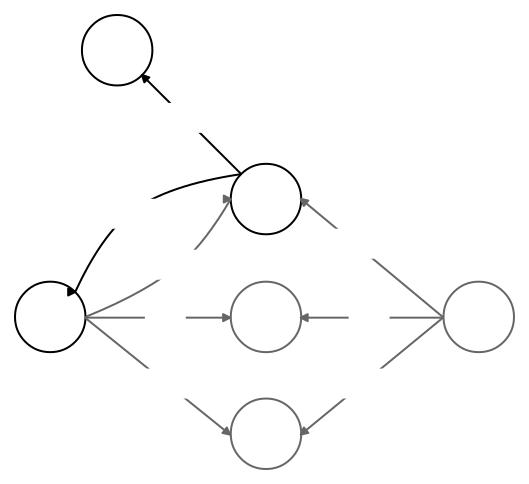
\includegraphics[width=0.65\textwidth]{content/unveiling/img/temporal_network}
\caption{Example of the resulting temporal network of two transactions: \textit{T1}(two inputs and three outputs) and \textit{T2}(one input and two outputs). Where the Output 1 of the \textit{T1}, is the Input 1 of \textit{T2}.}
\label{fig:temporalNetwork}
\end{figure}

\end{document}